\documentclass[11pt,addpoints]{exam}
\usepackage{enumitem}
\usepackage{amsfonts,amssymb,amsmath, amsthm}
\usepackage{graphicx}
\usepackage{systeme}
\usepackage{pgf,tikz,pgfplots}
\pgfplotsset{compat=1.15}
\usepgfplotslibrary{fillbetween}
\usepackage{mathrsfs}
\usetikzlibrary{arrows}
\usetikzlibrary{calc}
\pagestyle{headandfoot}
%\firstpageheadrule
\runningheader{Current}{}{Page \thepage\ of \numpages}
\runningheadrule
\author{Aaron GK}
\usepackage{geometry}
\geometry{
	a4paper,
	total={170mm,257mm},
	left=10mm,
	right=10mm,
	bottom=5mm,
	top=5mm,
}
\firstpagefooter{}{}{}
\runningfooter{}{}{}
\begin{document}
			\title{The Hall Effect}
			\maketitle
So far in electromagnetism, we have seen the effects of magnetism on moving charges and current carrying wires. As many phenomena in nature are symmetric, so is electromagnetism. As we get magnetism effects from moving charges and current carrying wires, we also get current from magnetism. One important example of this effect was observed by a physicist called \textbf{Edwin Hall}; a conductor moving perpendicular to a magnetic field induces a voltage.\\ \\
Consider a conductor moving perpendicular to a magnetic field as shown in the figure below(\textit{the field is perpendicular to the electron drift velocity and to the width of the conductor.}):
\begin{center}
	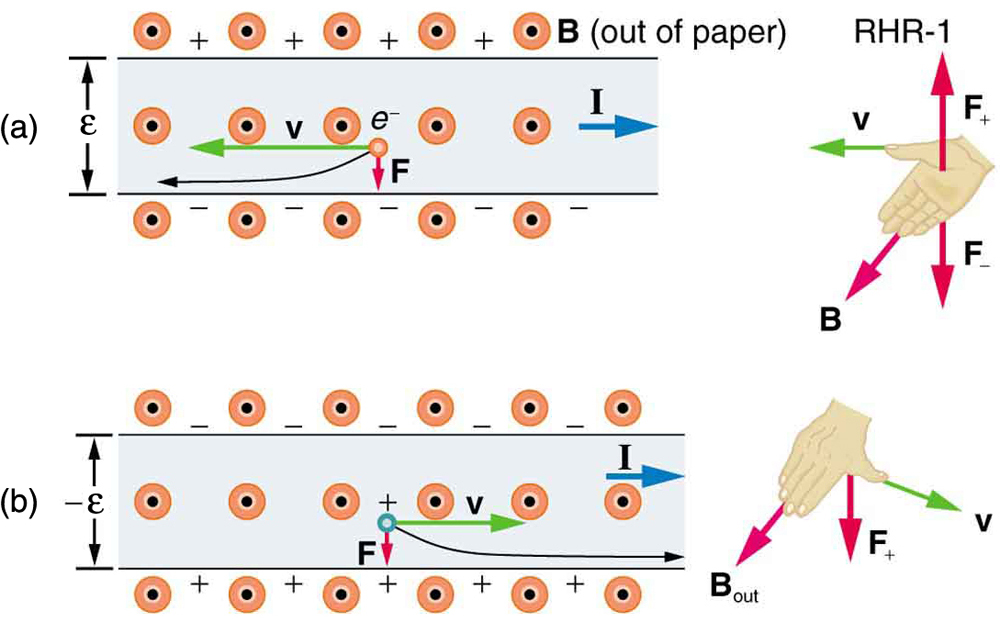
\includegraphics[scale=0.5]{hall_1}
\end{center}
 In part \textbf{(a)}, electrons carry the current and move to the left. In part \textbf{(b)}, positive charges carry the current and move to the right. Moving electrons feel a magnetic force toward one side of the conductor, leaving a net positive charge on the other side. This separation of charge creates a voltage $\varepsilon$, known as the Hall emf, across the conductor. The creation of a voltage across a current-carrying conductor by a magnetic field is known as the Hall effect. The Hall Effect has many applications in physics and other fields including precision measurement of magnetic fields and determination of charge carriers. \\ \\
 Although the magnetic force moves negative charges to one side, they cannot build up without limit. The electric field caused by the separation of the opposite charges on the opposite ends of the conductor opposes the magnetic force. Initially, the magnetic force is much greater than the electric force, but as more charges build up, they eventually become in a state of equilibrium.
 $$F_e=F_B$$
 $$qE=qvB$$
 $$E=vB$$
 Since the electric field is constant due to the magnetic field being constant, we can express the induced potential difference due to the separation of the charges as a distance function of the electric field. As we have seen early on in electrostatics, this can be done as follows:
 $$V=Ed$$
 The voltage here is the emf and the distance here is the distance between the polarized ends of the conductor. We can rewrite it as follows:
 $$\varepsilon=El$$
 $$E=\dfrac{\varepsilon}{l}$$
 We can then go back to the original equation and plugin the expression we got for the field in terms of the emf.
 $$\varepsilon=Blv$$
 It is important to note that both $B$, $l$ and $v$ are all mutually perpendicular.
\end{document}